\chapter{The design of a distributed computing project}
% Pu these two ines after every \chapter{} command
\vspace{-2em}
\minitoc

Chapter 4 introduces the concept of distributed computing by  giving its history and a summary of some well-known projects, together with their results and the frameworks they were built on. The different distribution frameworks that are available today will then be surveyed.  The working of Berkeley Open Infrastructure for Network Computing, in particular, will be examined in detail, as well as all the requirements for a BOINC project.  The chapter will conclude in specifying the design choices neccessary to create a  BOINC project for the enumeration of main classes of \lat s, for example how to break the search tree up into workunits, how to assign workunits to a user based on system specifications etc.

\section{A brief history of public-resource computing}
In John Brunner's 1975 science-fiction novel, \emph{The Shockwave Rider} \cite{brunner}, the main character creates a "tapeworm" program which was able to propagate itself thro	ugh a network of computers, replicating when needed and consuming resources wherever available. This type of program, capable of harnessing resources on any number of machines, piqued the interest of a group of researchers at Xerox's Palo Alto Research Center (which was famously also the home of the first graphical user interface) who set about creating a number of "worms" programs for controlling multi-machine performance measurements of their pioneering first Ethernet network \cite{worms}. 
Distributed computing systems were mainly confined to networks within organisations or academic departments for the following two decades, until  widespread public adoption of personal computers and the internet made it possible to involve the public in distributed computing, or what will be called \emph{volunteer computing}.

Anderson \emph{et al.} \cite{boincwiki} defines volunteer computing as a form of computing where both organizations and members of the public can donate unused computing resources to \emph{projects}, which are usually applications of a scientific or academic nature. Volunteer computing is built largely on trust and mutual goodwill as it is necessary that the volunteers trust the projects not to perform unapproved calculations with their resources and to guard their personal account details carefully. Similarly, although IP and email addresses may be linked to individual volunteers, volunteers remain largely anonymous and there are no disciplinary steps available against a volunteer who wilfully corrupts computations. The main advantages of volunteer computing are, firstly, that it provides access to at least part of the approximately 10 billion devices linked to the internet \cite{cisco, anderson2013} and, secondly, that it raises public awareness of scientific endeavours and provides a mechanism through which a project of large popular appeal but little funding may flourish \cite{boincwiki}.
Volunteer computing is somewhat similar to two other forms of distributed computing namely \emph{grid computing} and \emph{peer-to-peer} networks. Grid computing is generally considered a paradigm through with computing resources are shared within and between organizations in a mutually beneficial way, for example through desktop grids made up of  all the desktop computers within an organization. This has many things in common with volunteer computing but differs in that the "volunteers" are usually more reliable because of a lack of anonymity and the accompanying existence of disciplinary measures \cite{boincwiki, fostergrid}. The principles of peer-to-peer computing, on the other hand, is  perhaps best seen in file-sharing services such as Napster or torrents - data transfer takes place between computers without any form of coordination by central servers \cite{peer, peer2}. Volunteer computing relies on central servers hosting the project and it is not possible for two clients to communicate directly without coordination by the central server. 
 

There are, however, also many challenges involved with publicly distributed computing, for example, the platforms on which your application must be able to execute accurately are a lot more heterogeneous  and the network is likely to be much more unreliable than within a corporation or laboratory.   Despite these factors, scientists were increasingly interested in unlocking to the massive computing power locked away in the idle computer cycles of the public and two early volunteer computing projects, the Great Internet Mersenne Prime Search (GIMPS), which searches for very large Mersenne primes \cite{gimps}, and \texttt{distributed.net}, which facilitates brute-force decryption, were created in 1996 and 1997, respectively. 

GIMPS continues to this day and, according to the project's homepage, currently runs on $737\,759$ CPUs around the world, with an average annual throughput of 129.2 TFLOP/s. Mersenne primes of the form $2^n-1$ for integer  values of $n$ account for most of the very large prime numbers; the first Mersenne prime discovered with GIMPS, $2^{1\,398\,269}-1$ was found in November 1996 \cite{hayes} and the  forty-eight Mersenne prime, and the largest known prime number, $2^{57\,885\,161} -1$ was recently found on 25 January 2013 \cite{gimps}. \texttt{distributed.net} also remains active today and concerns itself with finding optimal Golomb rulers (combinatorial curiosities with application to the placement of radio antennas in astronomy) and deciphering encoded messages \cite{distnet}, a trend which, according to Hayes \cite{hayes}, started when RSA Data Security company issued a number of challenges in 1997, hoping to test whether their encryption systems are breakable and demonstrate the inefficiencies of rival schemes. Notable early successes were the breaking of RSA-129, which involved the factoring of a 129-bit number similar to those commonly used in the RSA encryption scheme and  took 600 volunteers eight months to do, and the decryption of a message encrypted with the Data Encryption Standard (DES), which was developed under US government sponsorship in the 1970s \cite{distnet}. 
Another early project, which has grown into one of the most influential volunteer computing projects, is   SETI@Home (Search for Extraterrestrial Intelligence), launched  in 1999 by a group of scientists from the University of California to examine radio waves picked up by a telescope operated by Cornell University and the National Science Foundation in Arecibo, Puerto Rico \cite{anderson:seti2002}. The project was very well received by the public and attracted millions of volunteers, by 2004 the average sustained processing power of the SETI@Home project was more than 70 TeraFLOPS (1 TeraFLOPS of computing power is equivalent to $10^{12}$ floating point operations per second), more than double the 35 TeraFLOPS of the most powerful supercomputer at that stage, the NEC Earth Simulator \cite{anderson2004boinc}.
 


According to Anderson \emph{et al.} \cite{anderson:seti2002}, the encouraging success of these early projects lead to a wider push for frameworks which could be used for public-resource or large-scale distributed computing. In 1999 the Global Grid Forum was formed as an umbrella corporation for a number of distributed projects collectively called \emph{The Grid} \cite{fostergrid} for resource sharing amongst research organizations, while many private organizations, including Platform Computing and United Devices were developing corporate systems for distributed storage and computation. The biggest milestone in the history of public-resource was, perhaps, the launch of \emph{Berkeley Open Infrastructure for Network Computing} (or BOINC) in 2004 \cite{anderson2004boinc}, spearheaded by David Anderson, who was the Chief Science Officer at the time at United Devices and also co-founder of the SETI@Home volunteer computing project. 

BOINC acts as middle-ware between the scientists and the public, handling the required network connections automatically and thereby drastically decreasing the difficulty of setting up a new project, providing scientists with a comprehensive \emph{application programming Interface} (API) with which to interact with volunteers and letting volunteers use the same client to connect to multiple volunteer computing projects. The first project to make use of BOINC was, unsurprisingly, SETI@Home and a large number of scientific projects followed with applications ranging from testing Einstein's theory of general relativity (Einstein@Home) \cite{eah} and finding new arrangements into which proteins may fold themselves (Folding@Home) \cite{fah} to the distributed rendering of animated films (BURP) \cite{burp}.

More than 80\% of currently active public-resource computing projects make use of BOINC  and a number of large organizations are making use of volunteer computing to further science in a myriad of different ways. Examples include IBM's \emph{World Community Grid} (WCG) initiative which serves the community by computing vaccines for malaria and modelling the earth's fresh-water supply \cite{wcg}, the LHC@Home project based at CERN which processes vast quantities of data obtained from experiments in the Large Hadron Collider \cite{lhcah}, as well as the Climatepridiction.net project which is based at Oxford University in the UK and models runs a number of different models estimating the effects of climate change \cite{cpdn}.

BOINC remains under active development by a group of software developers and project administrators. A BOINC client for Google's open-source mobile operating system Android has recently been released, thereby enabling the approximately 470 million Android smartphones in the market \cite{mobithinking}, many of which have two, four or even eight processors,      to take part in volunteer computing \cite{android}.

\section{Berkeley Open Infrastructure for Network Computing}
The main aim of BOINC is to simplify setting up a large-scale volunteer computing project and to minimize the time required to administrate the day-to-day running of the project.  With BOINC, for example, a single computer may, after a few weeks of work, serve as a server for a project involving thousands of volunteers, by reducing the entry cost in this way  it has enabled many scientists with wildly varying backgrounds and only moderate programming skills to take advantage of public resources for their computing, something which would not have been possible had it been necessary that they design the entire system themselves. According to Anderson \cite{anderson2004boinc},  secondary goals included support for a diverse set of applications and programming languages, allowing the sharing of resources between autonomous projects by letting volunteers simultaneously connect to a number of projects and assigning a priority to each project   and, finally, rewarding the volunteers in some way by measuring the resources contributed.


As enticing as  the advantages of public resource computing and BOINC in particular may seem, it is important to note that not all applications will work equally well within this model. For an application to be successful in  utilizing public resources, especially in the developing world where high-speed internet is still a rarity,  it is very important that an application firstly has a large computation to data ratio so that small data transfers to volunteers can lead to hours and hours of computations and, secondly, that the execution of the application be independently parallelisable. Some types of applications are discussed in \cite{anderson:pc} which seem particularly well suited to this type of distribution, for example the simulation of complex physical systems  where every simulation is independent of the others  or physical models with complex parameter spaces which must be explored. Random and genetic algorithms may also benefit from volunteer computing, as every independent trail can be performed by a different volunteer in the case of random algorithms, while for genetic algorithms every volunteer may receive an independent population of solutions to evolve from. A final category of projects, which has perhaps proven most successful in practice, involves the analysis of large amounts of data, for example from radio telescopes as in the case of SETI@Home, or  from the Large Hadron Collider in the case of LHC@Home.

 \subsection{Basic workflow and concepts of volunteer computing}

 
According to \cite{boincwiki}, a BOINC \emph{project} is a self-contained entity consisting of a \emph{database}, \emph{website}, \emph{applications}, \emph{workunits} and \emph{results}.

An application consists of a number of different executable programs, usually one for every \emph{platform}. Standard platforms are pre-defined in BOINC and are usually combinations of CPU architectures and operating systems \emph{e.g.} a 32-bit Intel processor running Windows or a 64-bit Intel processor running Linux. Knowing which platform a computation executes on is important for ensuring correct results, as different platforms handle floating-point operations in different ways.

A workunit is a computation that has to be performed. A workunit is associated with a specific application and has various attributes, \emph{e.g.} the names of its input files, the estimated time that it will run for, the resources required to complete it \emph{etc.} It was mentioned in \ref{histvol} that the results returned by volunteers may not necessarily be trusted, volunteer computing projects usually mitigate this risk through \emph{redundant computing}, which means that every workunit is computed multiple times and the results are compared for correctness. A \emph{result} may therefore be seen as a copy of a workunit which is sent to a volunteer for computation and once a certain number of results of a specific workunit, called a quorum, has been returned they are compared to find the definitive or \emph{ canonical} result for that workunit.
All workunits and results are stored in a database on the server, along with additional information regarding applications, workunits, volunteers and hosts. Distinction may be made between a volunteer, who creates an account with an email address and password when joining a project, and a host, which is the actual machine performing the computation. A single account may thus have a number of hosts associated with it, each running a version of the BOINC client which allows the host to attach to scientific projects. Note that credit is associated with an account, so that all hosts running under the same account earn credit in the same place.

Once a volunteer has attached or connected to a specific project through the client it may request work from the project's servers. 
A deamon running on the server called the scheduler takes the hosts resources into account and transmits suitable results, if any are available, after which the computation takes place on the host. 
Once the computation has finished the client on the host will  report the answers back to the server along with a new request for work. 
The received results are stored on the server until a quorum has been completed, after which they are checked for correctness or \emph{validated}, given credit for correct results and finally processed or \emph{assimilated}. 
In the meantime the host would have received new results for processing and the process, illustrated in Figure \ref{fig:workflow}, may be repeated as long as there are uncomputed results available.
\begin{figure}[htb]\label{fig:workflow}
\centering

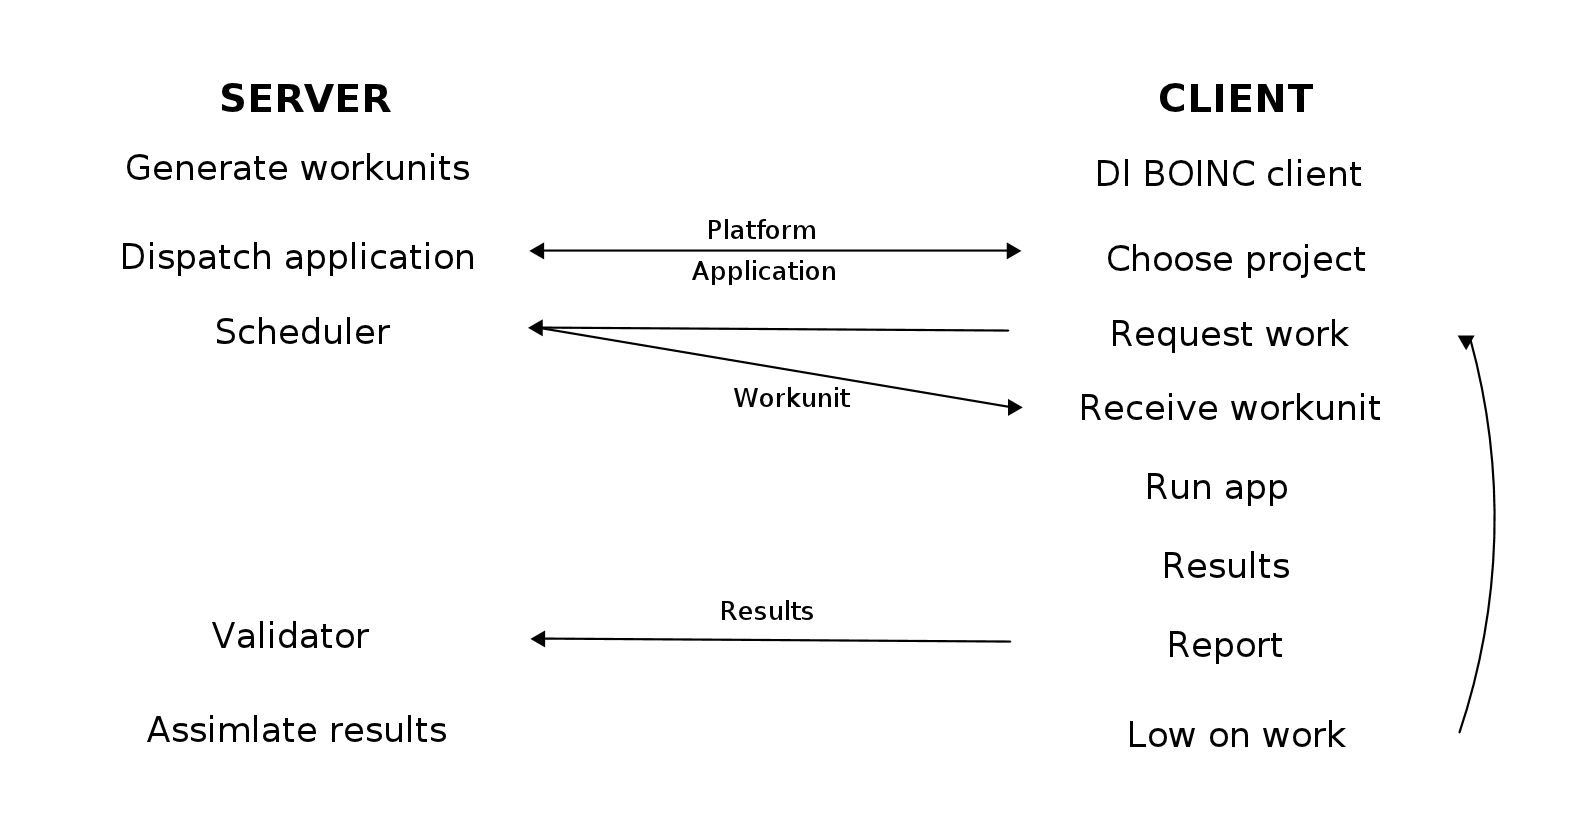
\includegraphics[width=14cm]{images/workflow}

\caption{Example workflow}
\end{figure}

\subsection{Grid-enabling a simple BOINC project}
A scientist attempting to turn an existing application into a volunteer computing project must  determine how the application will be parallelised, modify his existing application to make use of the BOINC API and finally provide the server-side deamons responsible for scheduling,  generating new workunits and validating and assimilating incoming results.
The first of these tasks, parrellelising the computation is highly application specific and has little to do with the structure and components of a BOINC project but it may be insightful to give further consideration to the BOINC API and the various deamons running on the server.
\subsubsection{The BOINC API}
The BOINC API provides a set of functions that firstly allow the client and the application to communicate and secondly improves portability of the application between different platforms.
An application must notify the client when it initialises through a call to \texttt{boincinit()} and return a value when terminating so that the client may track whether the computation was successful or not. 
The API also handles input and output, resolving logical names to actual filenames as specified in the workunit and providing wrappers for functions which execute differently on different platforms, for example a \texttt{boincfopen()} function which replaces the standard fopen call for opening functions so that on Windows hosts, where files may become temporarily locked, the function attempts to open the file multiple times within short succession and on Unix, where fopen() occasionally fails with a specific error code, it check for this error code and retries accordingly. 
\emph{Checkpointing}, or saving the current state of the computation in such a way that the computation may be resumed from that point, is very important in volunteer computing as there is no way of knowing when a host may be turned off or fail. Applications may choose their own minimum time between checkpoints, usually based on how long it takes to checkpoint, and may repeatedly call the method \emph{boinctimetocheckpoint()} to determine when to checkpoint. Checkpointing is also an example of a \emph{critical section} of an application, or a section which may not be interrupted by the client. 
BOINC  allows communication between the appliication and server through \emph{trickle messages}, small messages that are sent up from the client or down from the server and which has a very high priority. A trickle down message may for example be sent to notify an application that the result which it is computing is no longer needed and should be aborted, similarly a trickle-up message may be sent to the server to notify it that although a results has reached its deadline it is still being sunccessfully computed, in which case the original deadline should be extended.
The remainder of the API mainly focusses on providing methods which let the client register the time that the computation takes and monitor its progress, the full API along with a brief summary of every function as described in \cite{boincwiki, boincgit} may be found in Table \ref{tab:api}.
\begin{table} 
\caption{A selection of the parameters that may be specified in the output template, as found in \cite{boincwiki}}
\begin{tabular}{lp{11.6cm}}\toprule
 \multicolumn{2}{l}{\textbf{Output template options} \cite{boincwiki}   }\\ \cmidrule(r){1-2}
 \verb|name| & The physical file name of the output file\\
\verb|open_name| & The "logical name" by which the application will reference the file.\\
\verb|max_nbytes| & Maximum file size. If the actual size exceeds this, the file will not be uploaded, and the job will be marked as an error.\\
\verb|url| & the URL of the file upload handler. \\ 
\verb|no_delete| & If present, the file will not be deleted on the server even after the job is finished.\\
\verb|report_immediately| & If present, clients will report this job immediately after the output files are uploaded, otherwise they may wait up to a day. 
\\  \bottomrule
\end{tabular}\label{tab:api}
\end{table}
 
\subsubsection{Deamons}
The main task of the work generator is inserting new workunits or jobs into the project database. This may happen once, at the start of the project, in a number of discrete batches or continuously as results are returned from the volunteers. It is also possible to develop a web interface which allows for the remote submission of jobs.
Before implementing the work generator, however, projects must decide on templates for the workunits and results. These templates are XML files which provide  the application with the necessary information to compute the workunit and are typically re-used for millions of jobs. 
An input template may for example specify the name of the actual file to which the logical filename must be resolved, possible command-line arguments along with workunit attributes such as an estimate of its execution time, the resources required for the computation and the deadline by which the server expects to receive the result before re-issuing the workunit to a different host.  
Similarly, the output template defines the number of files returned to the server and where they are to be found or generated, a selection of the most important options that may be specified in the input and output templates may be found in Tables \ref{tab:intemplate} and \ref{tab:outtemplate}, respectively. The work generator ensures that the required files and templates are available before entering the workunit into the database. The BOINC API provides both a command-line tool and  a C/C++ method which inserts new jobs into the project database.
\begin{table} 
\caption{A selection of the parameters that may be specified in the input template, as found in \cite{boincwiki} }
\begin{tabular}{lp{11.5cm}}\toprule
\multicolumn{2}{l}{\textbf{Input template options }\cite{boincwiki} }\\ \cmidrule(r){1-2}
\verb|open_name| & The logical name of the file used in the application, \emph{e.g. `in'}.\\
\verb|command_line| & The command-line arguments to be passed to the main  application.  \\
\verb|rsc_fpops_est| &
An estimate of the number of floating-point operations required to complete the job, used to estimate how long the job will take on a given host.\\
\verb|rsc_fpops_bound| &
An upper bound on the number of floating-point operations required to complete the job. If this bound is exceeded, the job will be aborted.\\
\verb|rsc_memory_bound| &
An estimate of job's largest working set size. The job will only be sent to hosts with at least this much available RAM. If this bound is exceeded, the job will be aborted.
\\
\verb|rsc_disk_bound| &
A bound on the maximum disk space used by the job, including all input, temporary, and output files. The job will only be sent to hosts with at least this much available disk space. If this bound is exceeded, the job will be aborted.\\
\verb|rsc_bandwidth_bound| &
If nonzero, this job will be sent only to hosts with at least this much download bandwidth. Mainly used for jobs with very large input files. \\
\verb|delay_bound| &An upper bound on the time (in seconds) between sending a result to a client and receiving a reply.  If the client doesn't respond within this interval, the server 'gives up' on the result and generates a new result, to be assigned to another client.  
\\
\verb|min_quorum| &
The minimum size of a quorum. The validator is run when there are this many successful results. If a strict majority agree, they are considered correct. Set this to two or more if you want redundant computing.
\\
\verb|target_nresults| &
How many results to create initially. This must be at least \verb|min_quorum|. It may be more, to reflect the ratio of result loss, or to get a quorum more quickly.
\\
\verb|max_error_results| &
If the number of client error results exceeds this, the work unit is declared to have an error; no further results are issued, and the assimilator is triggered. This safeguards against workunits that cause the application to crash.
\\
\verb|max_total_results| & If the total number of results for this workunit would exceed this, the workunit is declared to be in error. This safeguards against workunits that are never reported (\emph{e.g.} because they crash the core client).
\\
\verb|max_success_results| & If the number of success results for this workunit exceeds this, and a consensus has not been reached, the workunit is declared to be in error. This safeguards against workunits that produce non-deterministic results.
\\
\verb|priority| &  Higher-priority work is dispatched first \\
\verb|size_class| & Used to define workunits of different sizes, for example in the case where the GPU version of an application is orders of magnitudes faster than the CPU version. \\ \bottomrule
\end{tabular} \label{tab:intemplate}
\end{table}

\begin{table} 
\caption{A selection of the parameters that may be specified in the output template, as found in \cite{boincwiki}}
\begin{tabular}{lp{11.6cm}}\toprule
 \multicolumn{2}{l}{\textbf{Output template options} \cite{boincwiki}   }\\ \cmidrule(r){1-2}
 \verb|name| & The physical file name of the output file\\
\verb|open_name| & The "logical name" by which the application will reference the file.\\
\verb|max_nbytes| & Maximum file size. If the actual size exceeds this, the file will not be uploaded, and the job will be marked as an error.\\
\verb|url| & the URL of the file upload handler. \\ 
\verb|no_delete| & If present, the file will not be deleted on the server even after the job is finished.\\
\verb|report_immediately| & If present, clients will report this job immediately after the output files are uploaded, otherwise they may wait up to a day. 
\\  \bottomrule
\end{tabular}\label{tab:outtemplate}
\end{table}

It is highly likely that a new project will, at least initially, make use of the default scheduler  provided along  with the BOINC source code.
The scheduler is responsible for accepting requests for work from hosts, assigning work to hosts based on a combination of their available resources, the estimated execution time of the available workunits and the historical accuracy of a host. Larger workunits are thus sent to hosts who historically return less erroneous computations and have more resources available in order to minimise the expected computation time that will be lost if a host returns an error after an extended period of   work.
Secondary objectives which may be included in the scheduler is finishing a specific batch of workunits as soon as possible or limiting the number of workunits that a host may receive on a single day to prevent hosts from repeatedly returning the same results and claiming credit for them.

The main task of the validator is to compare results for correctness. Care must be taken when comparing results from different platforms, for example, the end-of-line character is different between Windows and Linux making a character by character comparison of the output files impossible. If an application does a lot of floating-point operations projects may elect to enforce a measure called \emph{homogeneous redundancy} to ensure that results from the same workunit are assigned to identical platforms, alternatively fuzzy" comparisons may be made by comparing floating-point numbers with a degree of tolerance. A measure called \emph{adaptive replication} may also be used, which decides on the number of replications of a specific workunit based on the historical error rate of the host which was assigned the first result, if the host usually returns accurate results the probability of replication taking place for that workunit will be small.
Validation takes place by majority when a quorum of results have been received and marks a result, along with its associated output files, as the canonical result against which any other results of the same workunit are compared in order to determine whether it was computed successfully and deserves credit.
Two sample validators are provided with the BOINC source code, the first is mainly used for testing purposes and simply marks every received result as successful while the second does a bitwise comparison of output files.

Once results are verified they should be marked accordingly in the database so that they are not assigned to any further hosts, their input files may be deleted from the location where they were accessible to hosts and the canonical output files may be moved to a specific location.
The sample assimilator does exactly this and it is up to projects to decide what other post-processing tasks to perform on validated results.

Projects which make use of trickle messages must also provide a deamon to handle these messages. Trickle messages may for example be used by the application to periodically send its current computation state to the server  so that the server may   determine whether to assign partial credit for the work done up to the current point  or   to abort the computation based on some internal logic.

\subsection{Special types of applications}
In addition to the basic functionality BOINC allows applications to display graphics, execute on multiple cores or GPUs through OpenCL \cite{opencl}, and CUDA \cite{cuda} or even run entirely within a virtual machine. 
\subsubsection{Graphics applications}
Publicly-launched volunteer computing projects usually attempt to provide volunteers with some visualisation of the computation running on their machine, either as a screensaver or in a window which can be opened in the BOINC Client Manager. The main reason for providing graphics is to further engage the public in the goals and workings of a scientific project in order to increase involvement, examples of graphics provided by SETI@Home and WCG may be seen in Figure \ref{fig:boincgraphics}.
\begin{figure}[htb]\label{fig:boincgraphics}
\centering
\begin{minipage}{7.5cm}
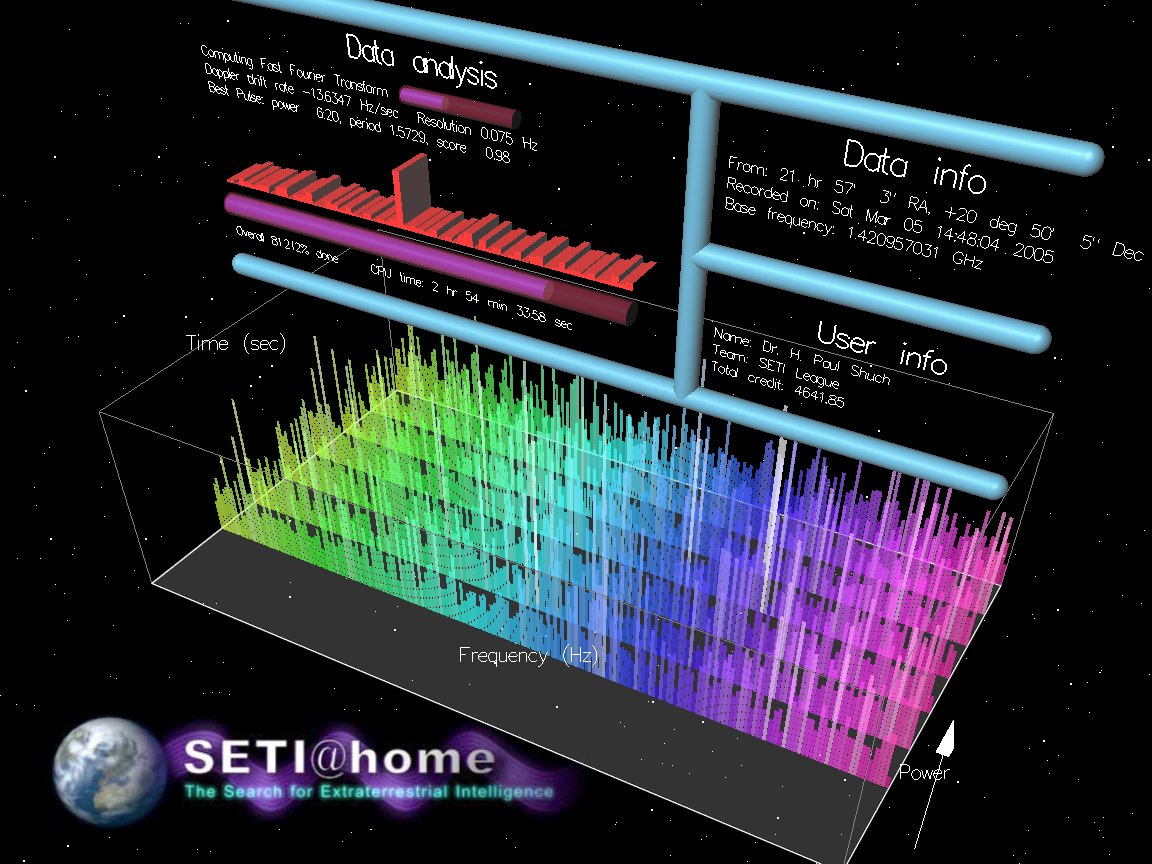
\includegraphics[width=7.5cm]{images/graphics1}
 \end{minipage} \hspace{.1cm}
\begin{minipage}{7.5cm}
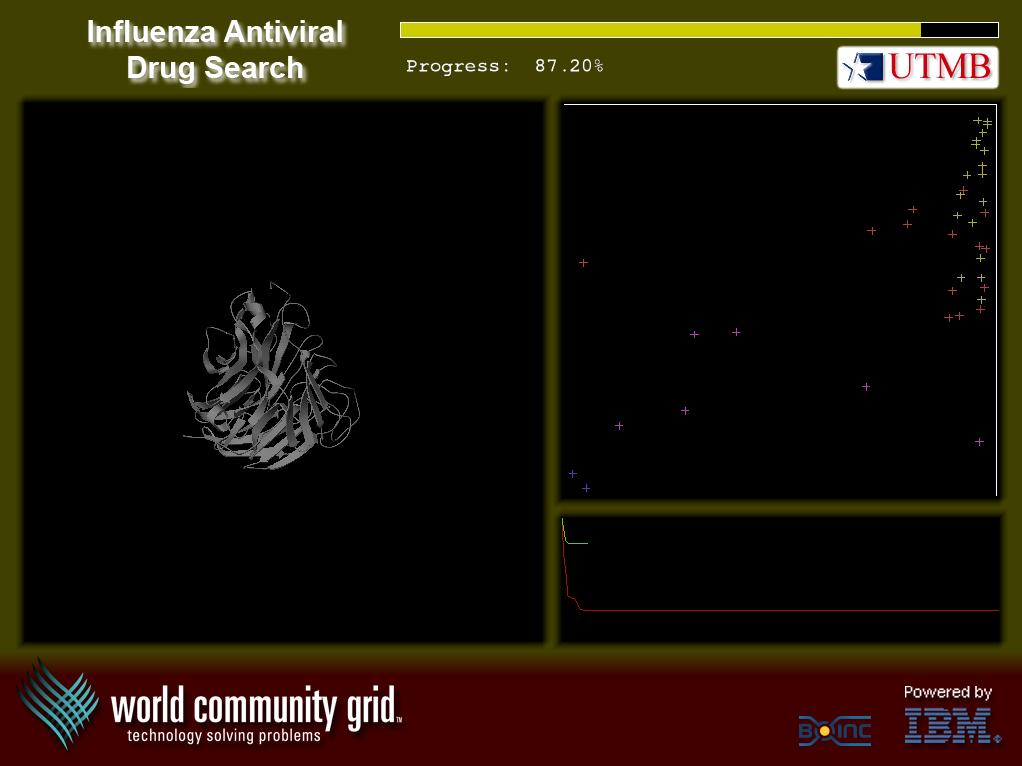
\includegraphics[width=7.5cm]{images/graphics2}
 \end{minipage}
\caption{Graphical applications provided by SETI@Home and WCG provide volunteers with an indication of the state of the current computation}
\end{figure}
  In a  recent survey of XXXX volunteers by IBM's World Community Grid project \cite{wcg}, however, XX\% of volunteers said that the graphics play a role in their involvement in a project \cite{wcg2013}, thereby casting some doubt on the actual benefit of graphical applications. Graphics applications are usually separate from the main scientific application, built on  a specific  BOINC graphics library and makes use of OpenGL \cite{opengl} for displaying graphics. Communication with the main application takes place through shared memory, the main application would periodically store a representation of its current state and progress in  a block of memory which is accessible to the graphics application, from where it will be read and displayed. Graphics applications can also display static images, text or web-based graphics by opening a browser windows pointing to a specific URL.

\subsubsection{Muti-core and GPU applications}
CPU manufacturers have been dealing with the limit placed on CPU frequency by increasing the number of cores provided and it seems that this trend will continue for some time. In cases where the completion time of individual workunits want to be increased, or the memory footprint of the application is too large to allow a separate copy of the application to run on every core it may be desirable to have a multi-threaded application developed in OpenCL, MPI, OpenMP, CUDA or a number of other languages. BOINC also supports what it calls `coprocessors' or GPUs designed by NVIDIA, AMD or Intel. Available GPUs are reported to the scheduler by the BOINC client, which also keeps track of which instances on every GPU is currently allocated. To prevent system, failures GPU kernels are  executed within critical sections, which may not be killed by the BOINC client and  BOINC projects may define workunits of different size classes to compensate for the potentially dramatic difference in speed between CPU and GPU versions of the same applications adnd thereby ensure that a typical workunit will take approximately the same amount of time irrespective of the architecture on which it is executed.

\subsubsection{Applications which run inside virtual machines}
BOINC supports application which run entirely within virtual machines. This approach has two distinct advantages in that it provides the highest level of security for the host machine, as virtual machines cannot access or modify the host system and there is no need to build applications for different architectures as every application will run on a virtual computer with exactly the same runtime environment on any platform.  
There are however also some additional complexities which arise from using applications inside virtual machines such as the fact  that hosts require software such VirtualBox to mount the machine image, yet VirtualBox  is not currently available for all processors. GPU applications can not currently be run inside VirtualBox and not all processors are capable of running both 32- and 64-bit virtual machines, so images of both will have to be provided. Distributing the virtual machine image also increases the size of the first download to approximately 200Mb, which may be prohibitive for volunteers with limited bandwidth.

\subsection{Setting up a server and project maintenance}
As stated in \S \ref{}, a BOINC project consists mainly of a MySQL database, a directory structure and a configuration file which specifies the options, deamons and periodic tasks which must be performed and as such, it is possible to use almost any computer as a  BOINC server \cite{boincwiki}.

As with any server reliability and security is of the utmost importance, a server should at least be placed behind a firewall and have a reliable internet connection for connecting with volunteers, with a static IP address. Additional hardware measures which may  be taken to improve reliability  include an uninterrupted power supply, automatic backups adequate cooling and hot-swappable spares. Any Unix or Linux distribution may be used for setting up a server and  detailed instructions are available at \cite{boincwiki}. 
Alternatively a project may elect to host its server either on the Amazon Elastic Cloud Computing (EC2) service, which removes   potential concerns about hardware reliability and security, or host in within a virtual machine. A virtual machine image is available which has all the software packages required to set up a server, as well  as a number of installing and configuration scripts.  

Once a server has been set up a number of maintenance tasks must be performed regularly, \emph{e.g.} reviewing the deamon logs for errors, deleting files as they are no longer needed and archiving  and purging old jobs from the database to prevent the database from becoming to large. BOINC provides small programmes for all of these activities. Additionally it is possible that, due to the popularity of a project, a server may no longer be able to keep up with  the traffic generated by the volunteers, which will result in dropped connections, slow website access, deamons which fall behind and very slow database queries. A number of strategies are discussed in the BOINC documentation for upgrading the server in such scenarios, including upgrading the server hardware,  hosting the database on a separate server and  parallelising the deamons and scheduler so that multiple instances are constantly running.

\subsection{Security}
According to \cite{boincwiki} a number of security concerns arise from the inherently public nature of volunteer computing, chief amongst which are
\begin{itemize}
\item result falsification,
\item credit falsification,
\item denial-of-server attacks on the project servers, 
\item theft of project files or participant account information, including email addresses, and
\item the distribution of malicious executables.
\end{itemize}
Result and credit falsification may be limited b y making use of replication and validation and limiting the number of results a user may receive creit for in a single day. 
BOINC protects projects agains denial-of-service attacks, in which servers are overrun by requests and transfers from automated programs, by providing a size limit for every file that is uploaded to the server (refer to Table \ref{tab:outtemplate} in \S \ref{}) and making use upload certificates. Every project is responsible for protecting its own users' account information against theft and servers should be subjected to regular security audits. Successful attacks of this type has harmed the image of specific projects and volunteer computing in general very much. \cite{son}
The greatest security risk to volunteer computing project is the potential that a server may be broken into and used to distribute malicious executables to volunteers. In order to prevent this a code-signing software is used which signs every approved and secure application version as authenticate. The computer which is responsible for code-signing applications should be kept in `cold storage', in other words, physically secure and completely disconnected from the network to prevent attackers from breaking into it and authenticating their applications. 

\subsection{Challenges}
Decline in recent years, trouble breaking out of the core demographic of technically minded males. New initiatives such as cycles for change make use of social media platforms to engage a wider audience, indeed cycels for change boast an even number of male and female users. Also largely unexploited in Cihine, little hardware, hardware is not standardised, etc, languages.

\subsection{Basic workflow}

 
Specifics about rgidenabling, splitting up the search tree,  checkpointing, validating, workgenerations, handling inconsistent subtree sizes.1


\section{challenges}
demographics: 92\% male in \cite{anderson:pc}



\section{Chapter summary}